% pagebreak e pentru a termina de desenat toate pozele inainte...
\pagebreak
\section{Interfața de administrare}

	Interfața de administrare nu poate fi accesată dacă nu se cunoaște ori calea, ori dacă nu se navighează din cadrul vizualizării cererii (pentru client, acest pas reprezintă încărcarea pozelor) pe pagina principală.

	Pagina principală a interfeței de administrare se găsește la:

	\begin{verbatim}
	/admin/
	\end{verbatim}

	În momentul în care utilizatorul navighează la \textit{orice} parte a aplicației de administrare și nu este înregistrat, pagina apare ca în figura~\ref{fig:login}.
	\begin{figure}
		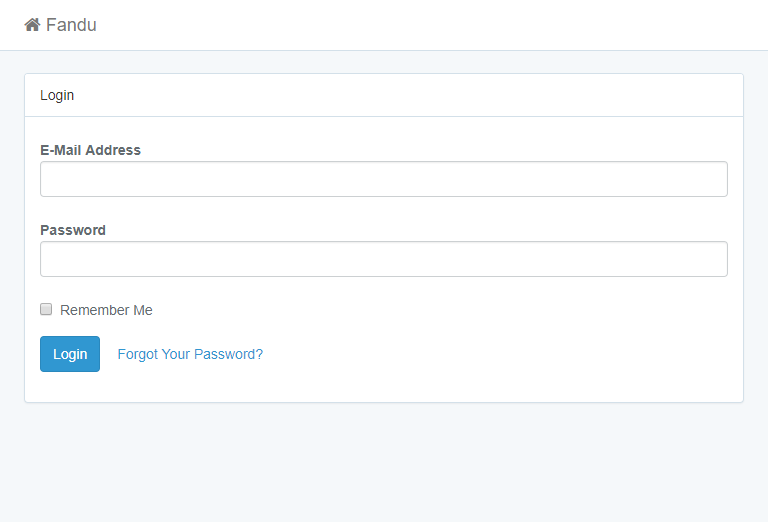
\includegraphics[width=\linewidth]{../imagini/login.png}
		\caption{Pagina de înregistrare pentru interfața de administrare}
		\label{fig:login}
	\end{figure}

	După ce utilizatorul introduce email-ul și parola sa corect în sistem, sistemul va naviga la pagina ce utilizatorul încerca să acceseze.

	Pagina principală a interfeței de administrare arată ca în figura~\ref{fig:home_page}.
	În cazul oricărei probleme, sunt lăsate datele mele de contact pentru a le remedia cât mai rapid.
	De aici, utilizatorul poate introduce rapid un număr de cerere de despăgubire folosind câmpul din bara de navigație.

	În pagina principală, se găsesc două grafice:
	\begin{enumerate}
		\item Primul se referă la cererile de despăgubire noi în această săptămână, raportat la numărul lor pe luna respectivă.
		\item Al doilea se referă la numărul total de decizii terminate, active și refuzate.
	\end{enumerate}

	Numerele folosite în aceste grafice apar atunci când se navighează cu cursorul deasupra lor.

	Bara de navigație conține toate modulele aplicației.

	\begin{figure}
		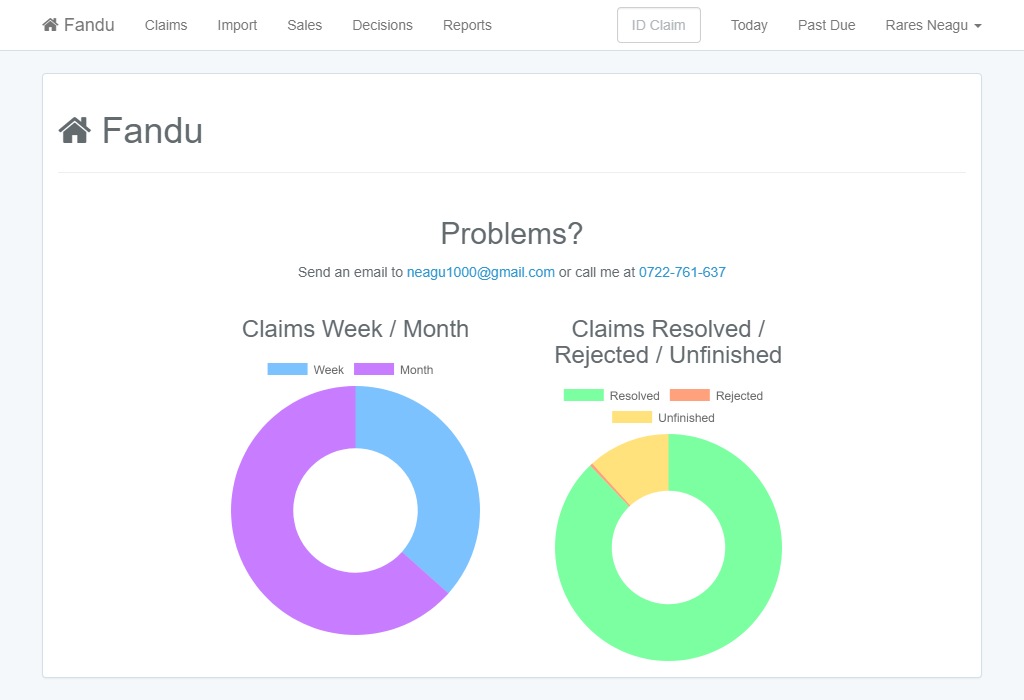
\includegraphics[width=\linewidth]{../imagini/home_page.png}
		\caption{Pagina principală a interfeței de administrare}
		\label{fig:home_page}
	\end{figure}

	\subsection{Modulul de administrare a cererilor de despăgubire}

	\begin{figure}
		\subfigure[Structura culorilor] {
			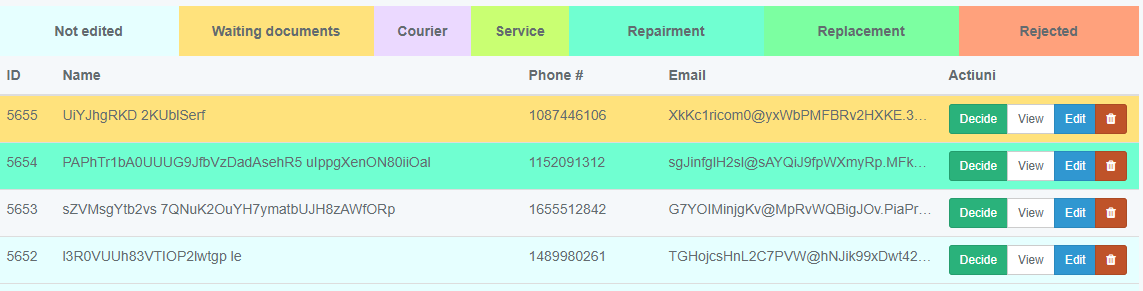
\includegraphics[width=\linewidth]{../imagini/color_coding.png}
			\label{fig:color_coding}
		}
		\subfigure[Filtrarea prin culori] {
			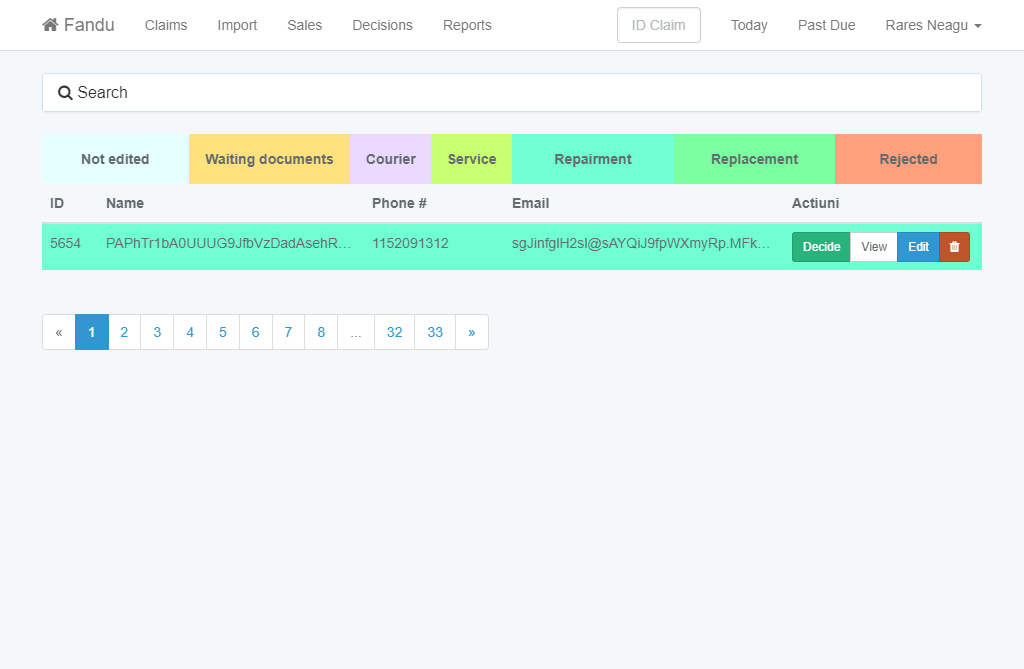
\includegraphics[width=\linewidth]{../imagini/claims_filtered.png}
			\label{fig:claims_filtered}
		}
		\subfigure[Căutarea cererilor] {
			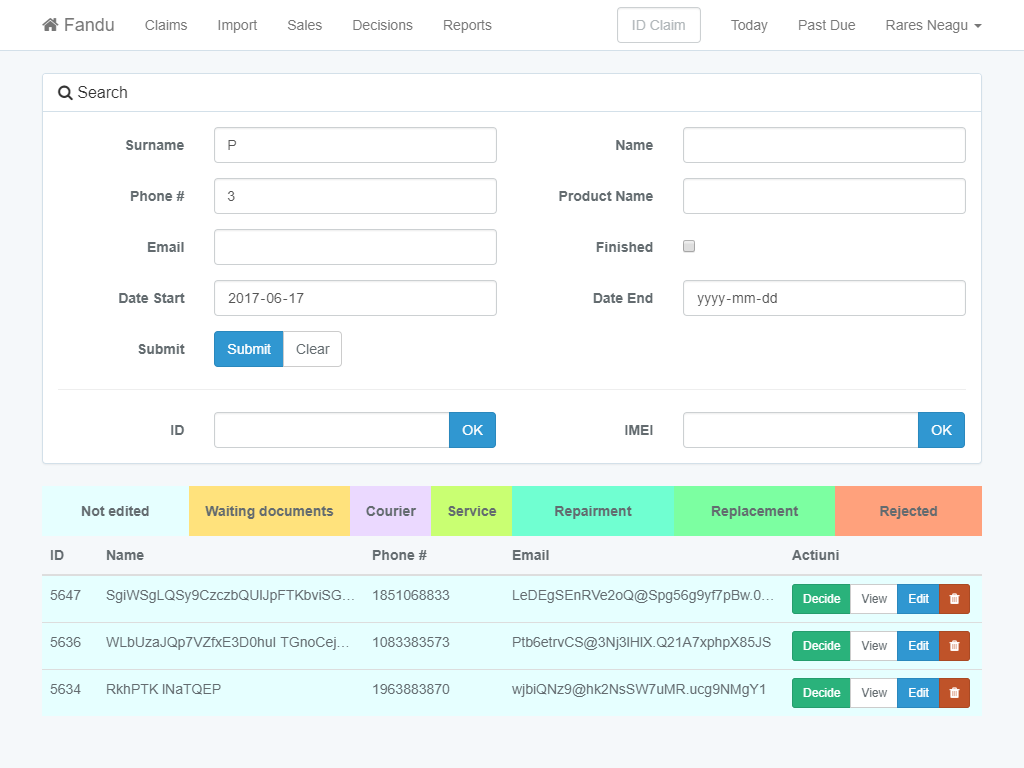
\includegraphics[width=\linewidth]{../imagini/claims_search.png}
			\label{fig:claims_search}
		}
		\subfigure[O cerere cu informații adiționale] {
			
\includegraphics[width=\linewidth]{../imagini/claims_tags.png}
			\label{fig:claims_tags}
		}
		\caption{Interfața administrării cererilor}
	\end{figure}


	Pe pagina principală a modului se vizualizează ultimele 100 cereri de despăgubire în funcție data sosirii lor în sistem.
	Fiecare cerere are patru butoane:
	\begin{enumerate}
		\item \verb|Decide| - pentru a naviga rapid la decizia cererii de despăgubire.
		Se va crea o decizie în cazul în care nu există.
		Dacă nu se poate construi automat decizia în funcție de numărul facturii, utilizatorul va fi rugat de a lega manual decizia de o vânzare sau de a construi el manual vânzarea în cauza lipsei acesteia.
		\item \verb|View| - vizualizarea cererii de despăgubire scrise de client.
		\item \verb|Edit| - modificarea cererii de despăgubire
		\item \verb|Delete| - iconița de gunoi reprezintă ascunderea cererii din interfața principală.

	\end{enumerate}

	Pentru a ajuta utilizatorul să identifice mai ușor starea cererilor, se reprezintă fiecare linie din tabel cu un sistem de culori, regăsit deasupra capului de tabel.
	Dacă se apasă un element din acesta, se filtrează cererile de pe pagina curentă după elementul respectiv.

	Figura~\ref{fig:color_coding} reprezintă un exemplu a datelor din tabel, figura~\ref{fig:claims_filtered} reprezintă cererile filtrate după „Repairment” (reparare), figura~\ref{fig:claims_search} arată sistemul de căutare în acțiune, iar figura~\ref{fig:claims_tags} prezintă o cerere cu informații adiționale.

	\subsubsection{Vizualizarea și modificarea cererilor}

	Pentru a modifica cererea, este obligatorie o decizie.
	Utilizatorul nu poate salva niciun câmp, după cum se vede în figura~\ref{fig:claims_edit}.

	După ce se adaugă decizia respectivă, utilizatorul poate scrie un mic detaliu despre cerere, a-i modifica starea, ce implicit modifică și starea deciziei (câmpul „Resolution”) și de a specifica când să-i aducă aminte aplicația despre cerere -- „Reminder” -- pentru a putea fi actualizate.
	Se pot observa aceste câmpuri în figura~\ref{fig:claims_edit_with_decision}.
	\begin{figure}
		\centering
		\subfigure[Fără o decizie - imposibil de modificat] {
			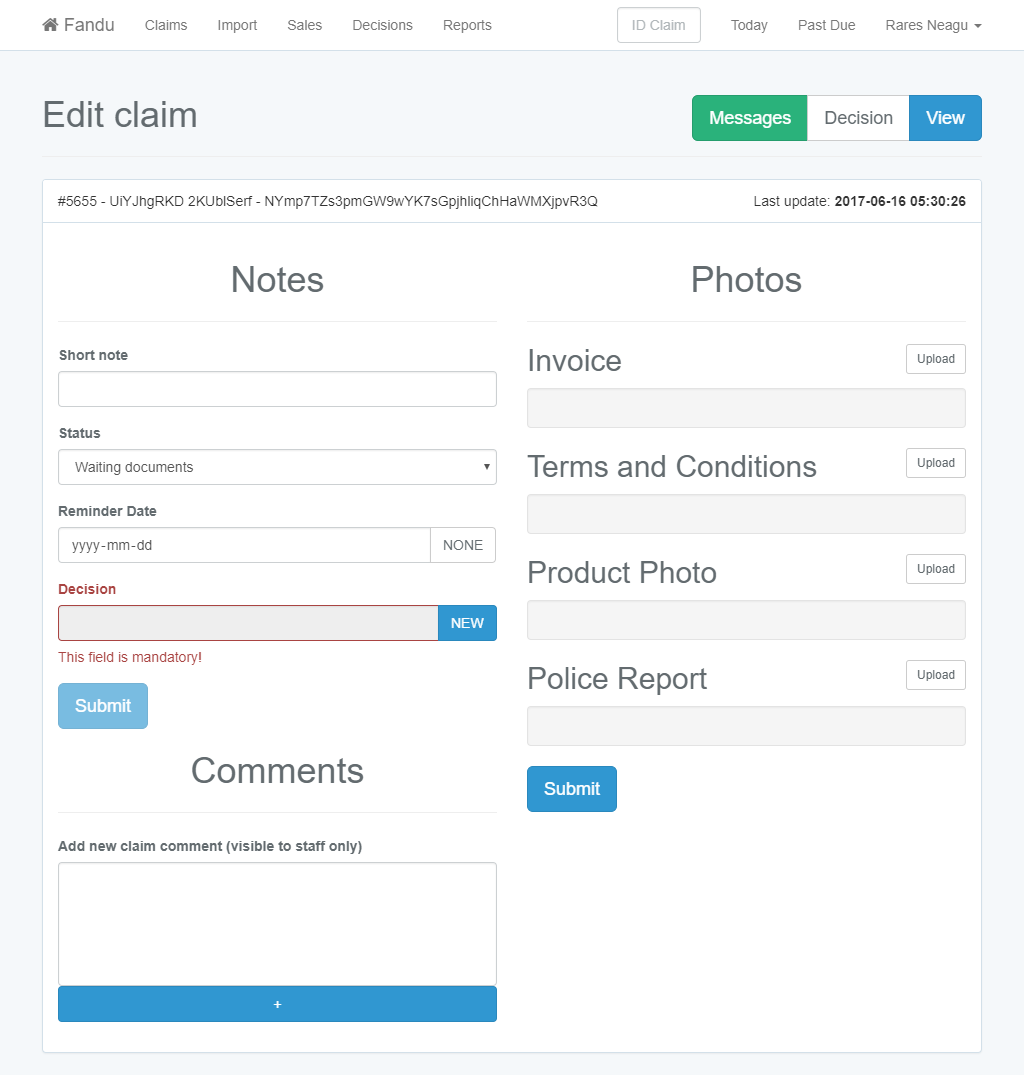
\includegraphics[width=0.4\linewidth]{../imagini/claims_edit.png}
			\label{fig:claims_edit}
		}
		\subfigure[Cu decizie - ușor de modificat] {
			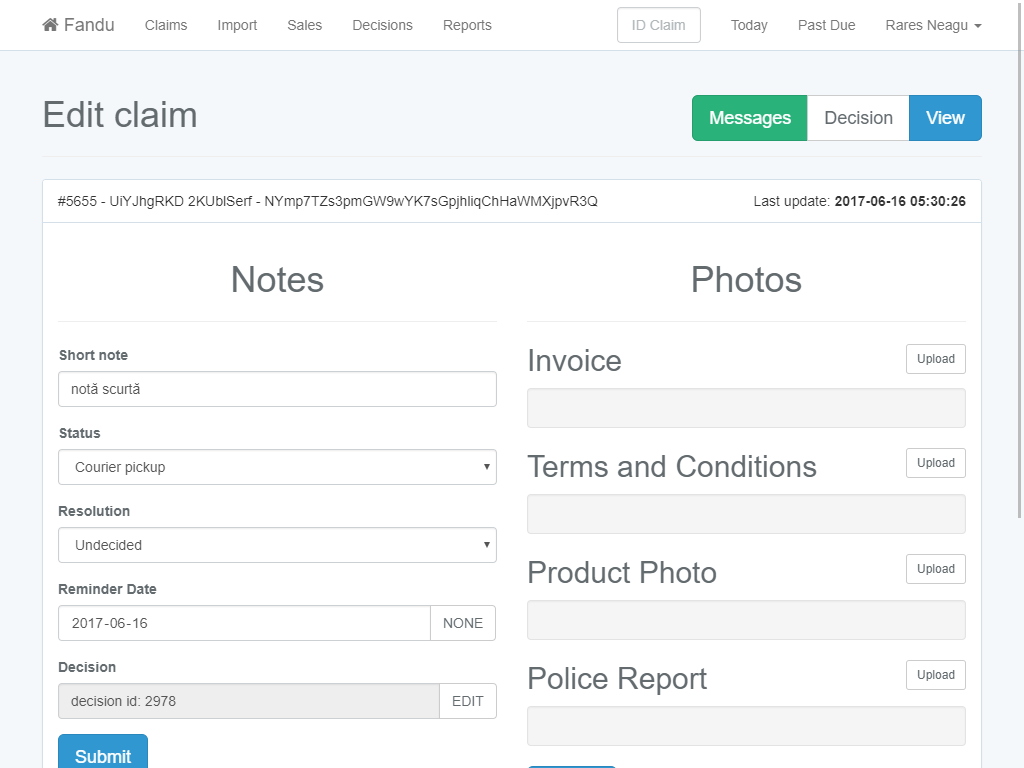
\includegraphics[width=0.4\linewidth]{../imagini/claims_edit_with_decision.png}
			\label{fig:claims_edit_with_decision}
		}
		\caption{Modificarea unei cereri}
	\end{figure}

	\subsubsection{Aducerea aminte a cererilor}

		Pentru că clienții au o perioadă de grație pentru a încărca pozele și pentru că multă lume revine ulterior cu ele, sistemul în meniul principal are două butoane:
		\begin{enumerate}
			\item \verb|Today| - Cererile ce trebuiesc actualizate exclusiv azi.
			\item \verb|Past Due| - Cererile ce trebuiau actualizate, aranjate după când trebuiau actualizate.
		\end{enumerate}
		Ambele secțiuni arată precum figura\ref{fig:claims_reminders}.
		\begin{figure}
			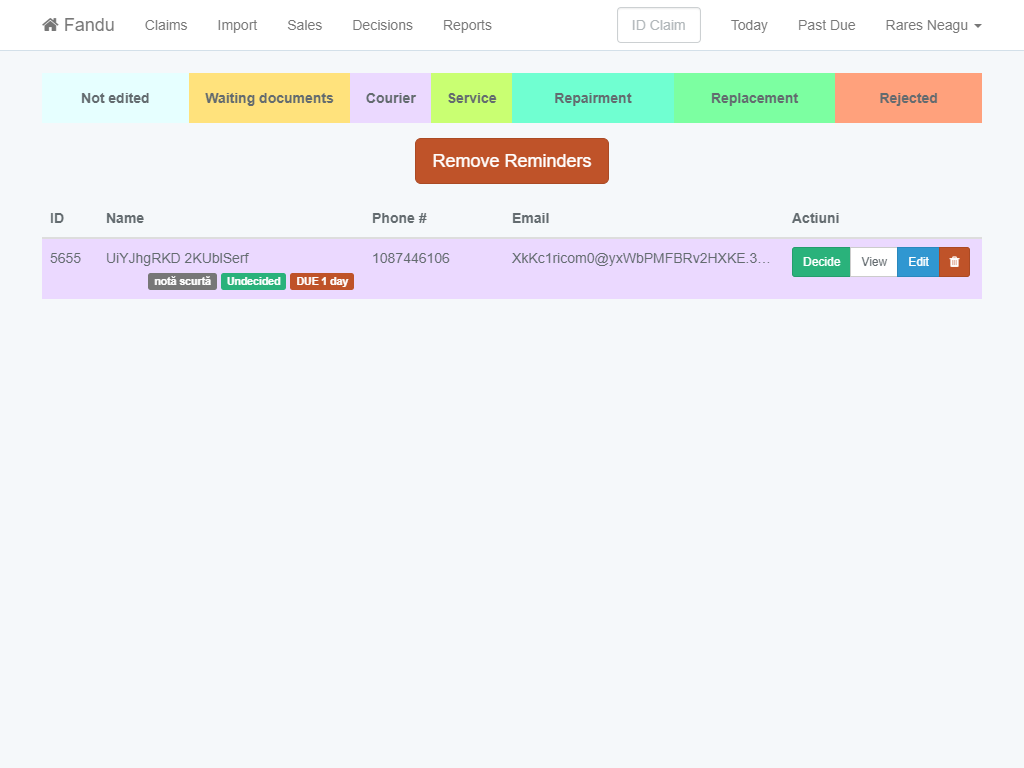
\includegraphics[width=\linewidth]{../imagini/claims_reminder_view.png}
			\caption{Sistemul de aducere aminte a cererilor de despăgubire}
			\label{fig:claims_reminders}
		\end{figure}
		S-a adăugat și butonul de șterge automată a câmpului  „Reminder”.

	\subsection{Modulul introducerii datelor în sistem}

		Introducerea datelor în sistem se face prin butonul „Import” din bara de meniu.
		Apar astfel două panouri, conform figurii~\ref{fig:imports}:
		\begin{enumerate}
			\item \verb|Weekly sale import| - Introducerea raportului principal aplicației. Se va trimite email de confirmare utilizatorilor aplicației, precum cel din~\ref{fig:message_mail_weekly_import}.
			\item \verb|Custom imports| - Introducerea datelor dinaintea aplicării sistemului în funcțiune pentru compania de asigurări.
		\end{enumerate}

		Se vor dezvolta propriile șabloane, ajustate nevoilor fiecărei companii ce folosește acest sistem de gestiune.

		\begin{figure}
			\centering
			\subfigure[Sistemul de introducere a datelor] {
			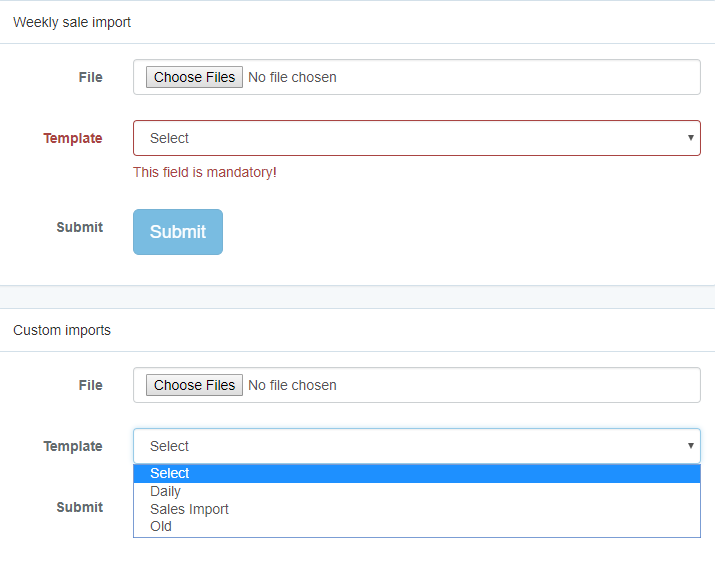
\includegraphics[width=0.6\linewidth]{../imagini/imports.png}
				\label{fig:imports}
			}
			\subfigure[Mesaj trimis utilizatorilor sistemului în momentul adăugării datelor în sistem] {
				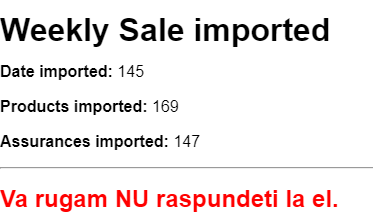
\includegraphics[width=0.2\linewidth]{../imagini/message_mail_weekly_import.png}
				\label{fig:message_mail_weekly_import}
			}
			\caption{Introducerea datelor}
		\end{figure}

		După momentul încărcării, utilizatorul trebuie să aștepte finalizarea introducerii datelor.

		Sistemul are grijă în cazul introducerii unui fișier duplicat, precum se vede în figura~\ref{fig:import_duplicate}, pentru că s-a încercat re-introducerea, din greșeală, aceluiași raport introdus cu succes în figura~\ref{fig:import_great}.

		\begin{figure}
			\centering
			\subfigure[Exemplu la introducerea cu succes a datelor] {
			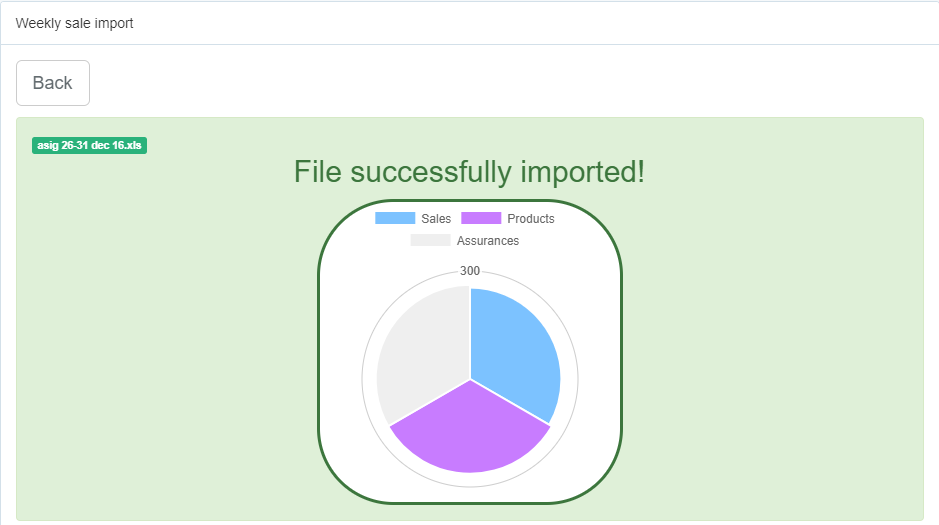
\includegraphics[width=0.4\linewidth]{../imagini/import_great.png}
				\label{fig:import_great}
			}
			\subfigure[Exemplu la încărcarea unui duplicat] {
				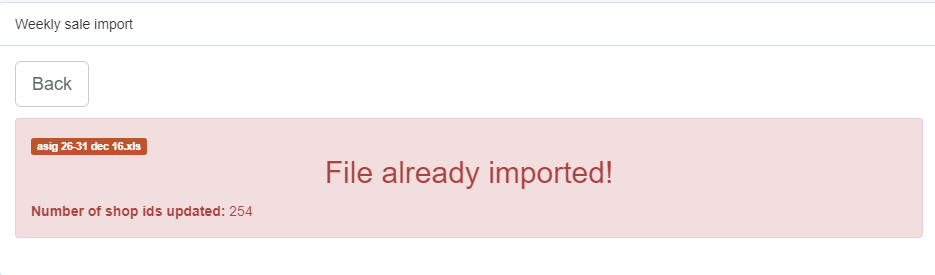
\includegraphics[width=0.4\linewidth]{../imagini/import_duplicate.png}
				\label{fig:import_duplicate}
			}
			\caption{Rezultate posibile la introducerea datelor în sistem}
		\end{figure}

	\subsection{Sales}
		search coloane, access rapid
		buton de remove / remove all logic
		\subsubsection{View}
				poti sa adaugi product
				poti sa stergi product
				poti sa adaugi assurance
				poti sa stergi assurance
	\subsection{Decisions}
		quick search
		detailed search
		de ce poti sa stergi - pentru ca daca nu ai asociat sale-ul corect, poti sa dai undo fara sa sufere nimic baza de date.
		\subsubsection{View}
				claim / messages / add old decision
				edit claim in urma analytics
				campurile explicate
				calculatorul
	\subsection{Reports}
		type of export (deprecated csv / excel)
		date start / end
		progress bar
		metadata when loading - especially yearly reports
		chunking
